%%% Template originaly created by Karol Kozioł (mail@karol-koziol.net) and modified for ShareLaTeX use

\documentclass[a4paper,11pt]{article}

\usepackage[T1]{fontenc}
\usepackage[utf8]{inputenc}
\usepackage{graphicx}
\usepackage{xcolor}

\renewcommand\familydefault{\sfdefault}
\usepackage{tgheros}
\usepackage[defaultmono]{droidmono}

\usepackage{amsmath,amssymb,amsthm,textcomp}
\usepackage{enumerate}
\usepackage{multicol}
\usepackage{tikz}
\usepackage[section]{placeins}

\usepackage{geometry}
\geometry{left=25mm,right=25mm,%
bindingoffset=0mm, top=20mm,bottom=20mm}


\linespread{1.3}

\newcommand{\linia}{\rule{\linewidth}{0.5pt}}

% custom theorems if needed
\newtheoremstyle{mytheor}
    {1ex}{1ex}{\normalfont}{0pt}{\scshape}{.}{1ex}
    {{\thmname{#1 }}{\thmnumber{#2}}{\thmnote{ (#3)}}}

\theoremstyle{mytheor}
\newtheorem{defi}{Definition}

% my own titles
\makeatletter
\renewcommand{\maketitle}{
\begin{center}
\vspace{2ex}    
{\huge \textsc{\@title}}
\vspace{1ex}
\\
\linia\\
\@author \hfill \@date
\vspace{4ex}
\end{center}
}
\makeatother
%%%

% custom footers and headers
\usepackage{fancyhdr}
\pagestyle{fancy}
\lhead{}
\chead{}
\rhead{}
\lfoot{}
\cfoot{}
\rfoot{Page \thepage}
\renewcommand{\headrulewidth}{0pt}
\renewcommand{\footrulewidth}{0pt}
%

% code listing settings
\usepackage{listings}
\lstset{
    language=Python,
    basicstyle=\ttfamily\small,
    aboveskip={1.0\baselineskip},
    belowskip={1.0\baselineskip},
    columns=fixed,
    extendedchars=true,
    breaklines=true,
    tabsize=4,
    prebreak=\raisebox{0ex}[0ex][0ex]{\ensuremath{\hookleftarrow}},
    frame=lines,
    showtabs=false,
    showspaces=false,
    showstringspaces=false,
    keywordstyle=\color[rgb]{0.627,0.126,0.941},
    commentstyle=\color[rgb]{0.133,0.545,0.133},
    stringstyle=\color[rgb]{01,0,0},
    numbers=left,
    numberstyle=\small,
    stepnumber=1,
    numbersep=10pt,
    captionpos=t,
    escapeinside={\%*}{*)}
}

%%%----------%%%----------%%%----------%%%----------%%%

\begin{document}

\title{\textbf{Brain Science Study} Part \textnumero{} 1}

\author{Nirupam Bidikar-1878058, Akshit Tandon-1792038, Rahul Raj Mogili-1900425}

\date{03/08/2020}

\maketitle

% -------------- Analysis 1 --------------- %
\section*{Analysis 1}

Construct the probability distribution function of the year of first publication of faculty.

\begin{lstlisting}[label={list:first},caption=Probability distribution function calculated]
author_data <- read.csv("brain_author.csv")
pub_year <- author_data %>% filter( min_pub_year > 1960) %>% select(min_pub_year)

g <- ggplot( pub_year,aes(min_pub_year)) + ggtitle("PDF for First Publication year of Faculty") + labs(y = "PDF",x = "Year" ) + geom_histogram(aes(y = ..density..),binwidth = 2, colour = "black", fill = "white") + geom_density(alpha=.2, fill="#FF6666")
g
\end{lstlisting}

% uploading the image of distribution of first publications
\begin{figure}[htp]
    \centering
    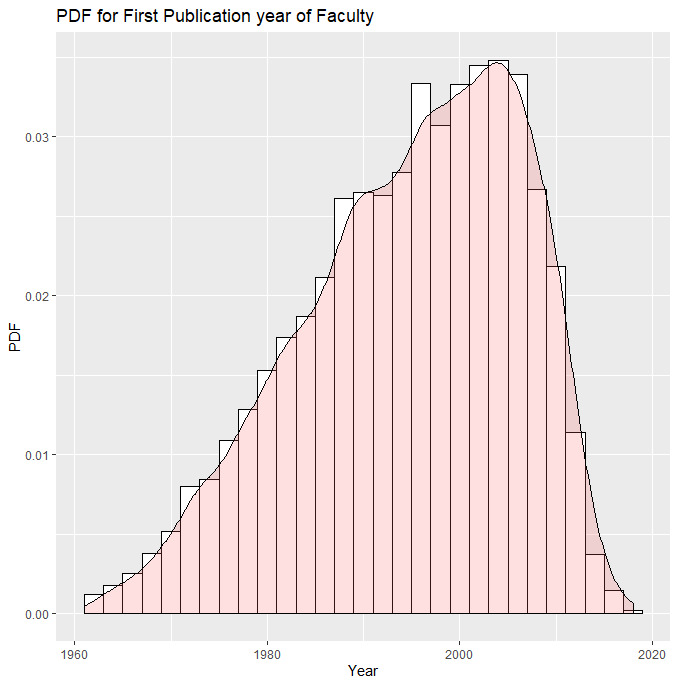
\includegraphics[width=10cm, height=10.5cm]{PDF_firstPub.jpeg}
    \caption{Probability Distribution Function of first year publications}
    \label{fig:PDF_firstcite}
\end{figure}


% problem 1 
The results indicate that we find a few outliers before the year 1960 which is statistically non relevant in this case study.

The number of publications from the above Probability Distribution Function gradually increases from the year 1960 up and until 2006, peaking at the year 2004. After the year 2006, the number of publications plummets till the time the records were updated. We also observe that the distribution is slightly skewed to the right with the later half of the distribution has more weight than the former.

The implementation of it can be found in the code snippet above.  We load the author data and filter it to select minimum publishing year as 1960. We then use the histogram and density functions from ggplot to plot the PDF.


% -------------- Analysis 2 --------------- %
\section*{Analysis 2}

Construct the probability distribution function of the total citations of faculty.

\begin{lstlisting}[label={list:second},caption=PDF calculated of the total citations of faculty]
total_citations <- author_data %>% filter(min_pub_year > 1960 && citations != 0) %>% select(citations)
transform <- log(1+total_citations)
g <- ggplot(transform,aes(citations)) + ggtitle("PDF for Total Citations of Faculty") + labs(y = "PDF",x = "Total Citations" )+ geom_histogram(aes(y = ..density..), binwidth = 0.5, colour = "black", fill = "white") + geom_density(alpha=.2, fill="#FF6666")
g
\end{lstlisting}

% uploading the distribution of total citations

\begin{figure}[htp]
    \centering
    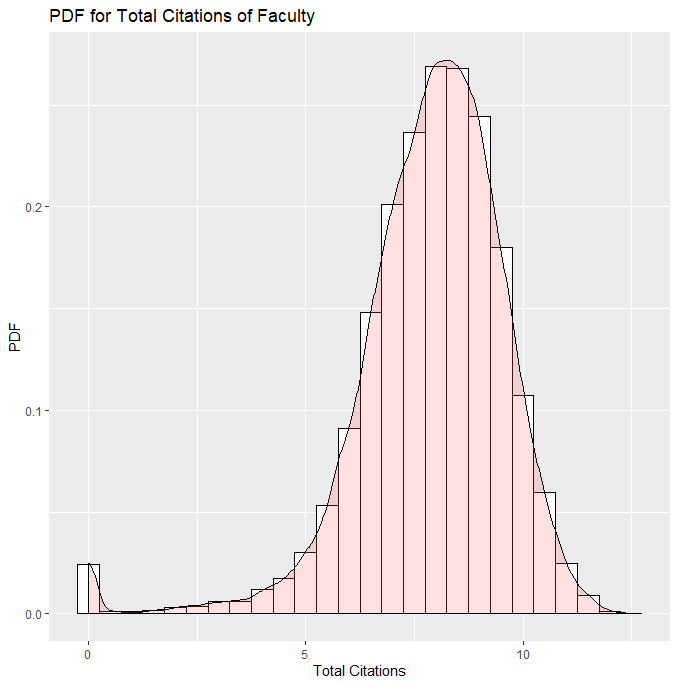
\includegraphics[width=10cm]{PDF_totalCitations.jpeg}
    \caption{Probability Density Function of total citations of faculty}
    \label{fig:galaxy}
\end{figure}

% problem 2 
We are using a log operator for this analysis to help plot the Probability Distribution Function.
The Probability Distribution Function is almost normally distributed. The implementation can be found in the code snippet above. We load the author data and filter it avoiding all rows with 0 citations and minimum publishing year as 1960. We use the previously used plotting functions to plot the graph.

% -------------- Analysis 3 --------------- %
\section*{Analysis 3}

Cluster the subject areas of faculty using the Louvain algorithm (k=5)

\begin{lstlisting}[label={list:first},caption=Cluster using Louvain algorithm]
publication_cat <- read.csv("brain_publication_areas.csv")
publication_cat <- unique(publication_cat)

#forming the edge list for the graph
combs <- inner_join(publication_cat,publication_cat, by="eid")
combs_alt <- combs %>% filter(!area.x == area.y)

#creatnig a graph from the edge list
g <- graph_from_data_frame(d = combs %>% select(area.x,area.y), directed = FALSE)

#clustering
clusters <- cluster_louvain(g)

area_to_cluster_map <- cbind(V(g)$name,clusters$membership)
colnames(area_to_cluster_map) <- c("area", "cluster")
area_to_cluster_map <- as.data.frame(area_to_cluster_map)
allclusters <- area_to_cluster_map
area_to_freq_map <- as.data.frame(table(publication_cat$area))
colnames(area_to_freq_map) <- c("area", "freq")

# selecting top 5 clusters 
y <- clusterdata %>% group_by(cluster) %>% add_tally(sort=TRUE) %>% select(cluster,n)
y <- unique(y)
top5 <- c(7,3,1,2,5)

merged_areas <- merge(area_to_freq_map, area_to_cluster_map, by = "area")
merged_areas <- merged_areas %>% filter(merged_areas$cluster %in% top5)
write.csv(merged_areas, "final_clusters_w_freq.csv")

# to make a word cloud -->
# you need to change these 3 variables for every cluster based on your personal choice
cluster_num = 5
min_freq = 1
max_size = 1
clrs = "black"
particular_cluster <- filter(merged_areas, cluster == cluster_num)
wordcloud(words = particular_cluster$area,
          freq = particular_cluster$freq,
          scale = c(max_size,0.5),
          min.freq = min_freq,
          max.words = Inf,
          random.order = FALSE,
          rot.per = .0,
          ordered.colors = TRUE,
          
          use.r.layout = FALSE)
\end{lstlisting}

Out of 330 topics and 11 clusters, the top 5 clusters we get are:

\begin{enumerate}[1.]
\item Neurology
\item Electrical and Electronic Engineering
\item Environmental Chemistry
\item Immunology
\item Cognitive Neuroscience
\end{enumerate}
We encountered difficulty in making the graph for the clustering algorithm and we noticed that a main cluster was getting split into two separate clusters which was the biochemistry cluster.
\begin{figure}[!htb]
    \centering
    
\includegraphics[width=10cm]{1.jpeg}
    \caption{Word Cloud 1}
    \label{fig:galaxy}
\end{figure}

\begin{figure}[!htb]
    \centering
    
\includegraphics[width=10cm]{2.jpeg}
    \caption{Word Cloud 2}
    \label{fig:galaxy}
\end{figure}

\begin{figure}[!htb]
    \centering
    
\includegraphics[width=10cm]{3.jpeg}
    \caption{Word Cloud 3}
    \label{fig:galaxy}
\end{figure}

\begin{figure}[!htb]
    \centering
    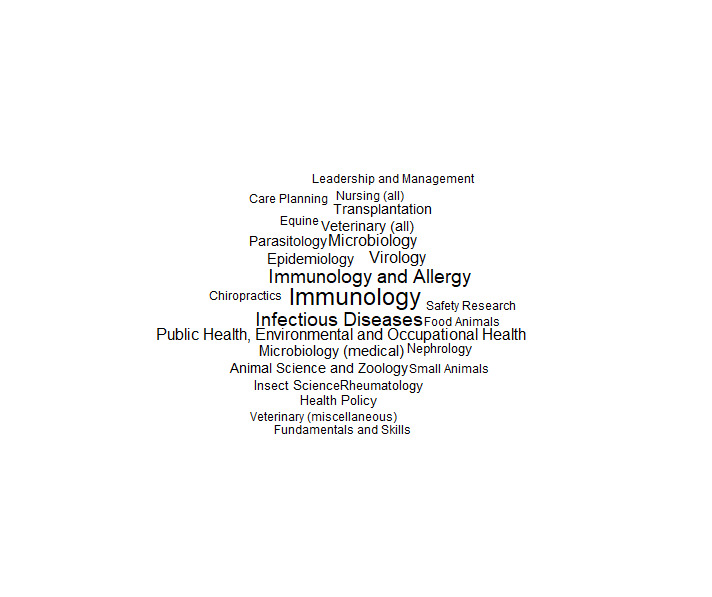
\includegraphics[width=10cm]{4.jpeg}
    \caption{Word Cloud 4}
    \label{fig:galaxy}
\end{figure}

\begin{figure}[!htb]
    \centering
    
\includegraphics[width=10cm]{5.jpeg}
    \caption{Word Cloud 5}
    \label{fig:galaxy}
\end{figure}


% problem 3 


% -------------- Analysis 4 --------------- %
\section*{Analysis 4}
Generate a bar plot of the number of publications per subject area per continent pre-2014, post-2014, and their difference.

\begin{lstlisting}[label={list:first},caption=Generating bar plot of the number of publications per subject]
clusterdata <- read.csv("final_clusters_w_freq.csv")
author <- read.csv("brain_author.csv")
pub_details <- read.csv("brain_publication_details.csv")
publication_cat <- read.csv("brain_publication_areas.csv")

combined_frame_1 <- merge(author, pub_details, by="scopus_id")
combined_frame_2 <- merge(combined_frame_1, publication_cat, by.x="eids",by.y="eid")
mergedData <- merge(combined_frame_2, clusterdata, by.x = "area",by.y ="area")
clusterHead <- sqldf("select area,cluster,max(Freq)from clusterdata group by cluster")
clusterHead
finalDataset <- merge(mergedData,clusterHead,by="cluster")
#this is a 2.6 GB file 
write.csv(finalDataset,"finalset.csv")

# Final Dataset to use after all joins

finalClusterSet <- read.csv("finalset.csv")
finalClusterSet <- finalClusterSet %>% select(eids,area.y,cip_title,scopus_id,pub_year,region,)

after_2014_q4 <- filter(finalClusterSet, pub_year > 2014)
before_2014_q4 <- filter(finalClusterSet, pub_year <= 2014)


#filtering values before and after 2014 and grouping based on subject area and region 
values_after_2014 <- after_2014_q4 %>% group_by(after_2014_q4$area.y, region) %>% filter(!is.na(region))  %>% add_tally()

values_before_2014 <- before_2014_q4 %>% group_by(before_2014_q4$area.y, region) %>% filter(!is.na(region)) %>% add_tally()


#plotting after 2014
g1 <- ggplot(values_after_2014, aes(x = region, y = n, fill =values_after_2014$area.y ))+
   geom_bar(stat = "identity",position=position_dodge())+ coord_flip() + ggtitle("Number of publications per subject area per continent post-2014") +
   labs(x = "region", y= "publications", fill="Subject Area")

#plotting beofre 2014
g2 <- ggplot(values_before_2014, aes(x = region, y = n, fill =values_before_2014$area.y ))+
   geom_bar(stat = "identity",position=position_dodge())+ coord_flip() + ggtitle("Number of publications per subject area per continent pre-2014") +
   labs(x = "region", y= "publications", fill="Subject Area")


grid.arrange(g1,g2)
\end{lstlisting}

\begin{figure}[htp]
    \centering
    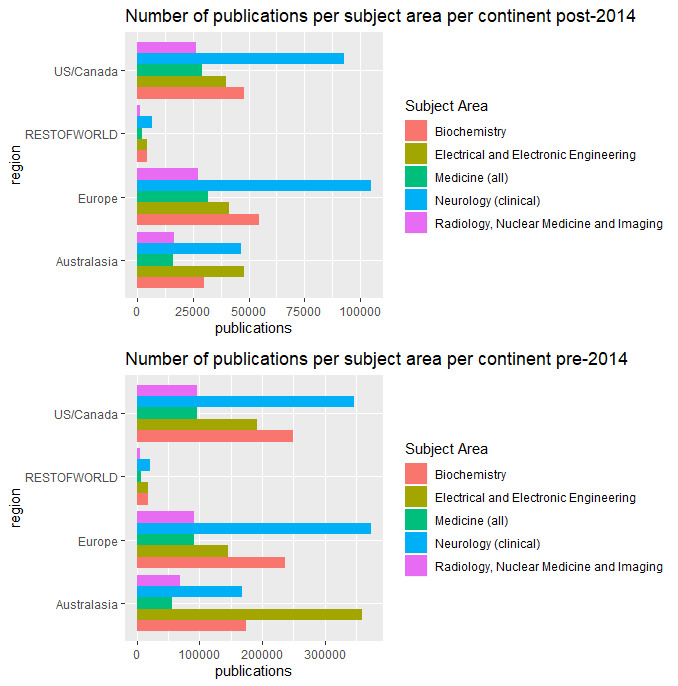
\includegraphics[width=10cm]{Q4_plot.jpeg}
    \caption{Number of Publications per continent pre and post 2014}
    \label{fig:galaxy}
\end{figure}

\begin{enumerate}[1.]
    
\item Neurology has most publications in all the regions except for Australia in both pre-2014 and post-2014. 

\item Meanwhile, Australasia has most number of publication in the subject area of Electrical and Electronic Engineering than any other region in both pre and post 2014

\item Europe has the most number of publications for a given subject area which is Neurology compared to any other continent.

\item The Rest of the World too has Neurology being the most number of publications.

\end{enumerate}

% problem 4


% -------------- Analysis 5 --------------- %
\section*{Analysis 5}

Generate a bar plot of the number of publications per CIP category per continent pre-2014, post-2014, and their difference.

\begin{lstlisting}[label={list:first},caption=Generating bar plot of the number of publications per CIP category per continent]
author_data <- read.csv("brain_author.csv")
pub_details <- read.csv("brain_publication_details.csv")

combined_frame <- merge(author_data, pub_details, by="scopus_id")
freq_cip <- as.data.frame(table(combined_frame$cip_title))
colnames(freq_cip) <- c("Cip_Title","Freq")
freq_cip_top6 <- sqldf("select * from freq_cip order by Freq Desc limit 6")
dd <- merge(combined_frame,freq_cip_top6 , by.x = "cip_title",by.y = "Cip_Title")
new_dd <- sqldf("select * from dd where region <> 'NA' ")

after_2014 <- filter(new_dd, pub_year > 2014) %>% filter(!is.na(region)) %>% filter(!is.na(cip_title))
grouped_after_2014 <- after_2014%>% group_by(after_2014$region, after_2014$cip_title) %>% add_tally()

before_2014 <-  filter(new_dd, pub_year < 2014) %>% filter(!is.na(region)) %>% filter(!is.na(cip_title))
grouped_before_2014 <- before_2014%>% group_by(before_2014$region, before_2014$cip_title) %>% add_tally()

comb_data <- merge(grouped_after_2014,grouped_before_2014, by.x="cip_title" , by.y="region")


# plot for after 2014 
g1 <- ggplot(grouped_after_2014, aes(x = region, y = n, fill = cip_title))+
  geom_bar(stat = "identity",position=position_dodge())+ coord_flip() +
    ggtitle("Number of publications per CIP per continent post-2014") + labs(x = "Region", y = "Publications", fill ="CIP")

#plot for before 2014
g2 <- ggplot(grouped_before_2014, aes(x = region, y = n, fill = cip_title))+
   geom_bar(stat = "identity",position=position_dodge())+ coord_flip() +
   ggtitle("Number of publications per CIP per continent pre-2014")  + labs(x = "Region", y = "Publications", fill ="CIP")

grid.arrange(g1,g2)

\end{lstlisting}

\begin{figure}[htp]
    \centering
    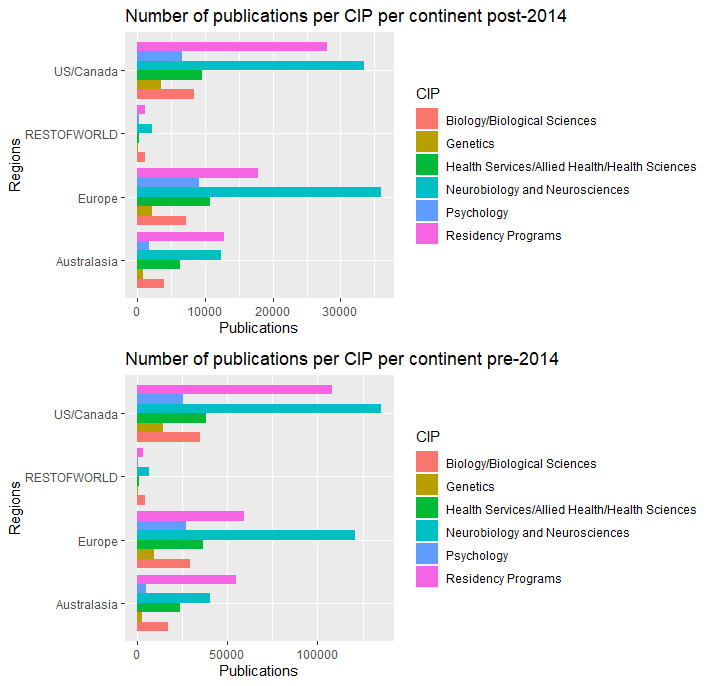
\includegraphics[width=15cm]{Q5_plot.jpeg}
    \caption{Number of Publications Pre and Post 2014}
    \label{fig:pre&post2014}
\end{figure}

% problem 5

\begin{enumerate}[1.]
    
\item The sum of all the CIP publications in US/Canada is greater than any other continent since the year 1960. 

\item Neurobiology and Neurosciences has the highest number of publications not only in Europe but all over the world pre-2014 whereas US/Canada takes the lead post-2014 in the same field overall.

\end{enumerate}




\end{document}
